\documentclass[12pt]{article}
\usepackage{geometry}
\geometry{a4paper, margin=1in}
\usepackage{graphicx}
\usepackage{booktabs}
\usepackage{hyperref}
\usepackage{natbib}
\bibliographystyle{apalike}
\usepackage{setspace}
\usepackage{multirow} 

\newcommand*{\MyHeaderPath}{.}% This path definition is also passed to inside the header files.
\newcommand*{\PathToAssets}{../assets}%
\newcommand*{\PathToOutput}{../output}%


\title{\textbf{FINM 32900 Final Project: Replicating Tables from \emph{Noisy Prices and Return-based Anomalies
in Corporate Bonds}}}


\author{Yuxuan (Ryan) Bai, Ximeng Deng, Yitong Wang, \\Yijing Zhang, Siying Zheng\\ \\The University of Chicago}


\date{February 2024}


\begin{document}

\maketitle

\begin{abstract}
This study endeavors to replicate Table 1 from the research article "Noisy Prices and Return-based Anomalies in Corporate Bonds" authored by Alexander Dickerson, Cesare Robotti, and Giulio Rossetti. Utilizing the TRACE database, we extracted data on corporate bonds and computed various metrics, including bid-ask bias, return, bid-ask spread, and credit spread, across different time periods and bond ratings. Our findings indicate that the replication results for Table 1 closely align with the statistics reported in the original study. However, it is imperative to acknowledge several challenges encountered during our analysis, which may have contributed to slight discrepancies between our results and those presented in the original paper.






\end{abstract}


\section{Introduction}
\subsection{Background}
The purpose of this project is to replicate table 1 from the paper "Noisy Prices and Return-based Anomalies in Corporate Bonds" written by Alexander Dickerson, Cesare Robotti, and Giulio Rossetti. As demonstrated by \cite{Dickerson2023Noisy},this paper tries to question the prevailing view that investors can earn usually high returns from certain patterns in corporate bond prices, such as return reversals and momentum. The authors debate these large gains are most likely a result of two factors: market microstructure noise an the use of arbitrary methods to limit extreme values in return data.


\subsection{Objective}
Our object is to replicate table 1 from page 11 from the paper. Table 1 in the paper is critical as it sets the foundation for the study's argument by presenting an analysis of bid-ask bias over time in the corporate bond market. The table includes time-series averages of cross-sectional means for daily bid-ask bias, return, bid-ask spread, and credit spread, all measured in basis points (bps). This information is crucial for the paper's thesis because it illustrates the extent of market microstructure noise — discrepancies in bond prices due to the mechanics of trading rather than changes in fundamentals — and how it can influence returns.


\section{Methodology}
\subsection{Data Sources}
The data source of Table 1 is the Wharton Research Data Services (WRDS) bond database, which integrates information from the Enhanced Trade Reporting and Compliance Engine (TRACE). We also utilize data from Mergent Fixed Income Securities Database (FISD) for details on bond issues. 

We followed the guidelines from \cite{OpenBondAssetPricing2023} website, specifically using the code from \cite{DickersonGithub2023} to generate our final replicated table. We used "MakeBondIntra\_Daily.py"  (renamed as "load\_trace.py") to generate the price and volume data. 

We apply the following filters to select bonds from WRDS bond database:

\begin{enumerate}
    \item Remove investment grade (IG) rated bonds that have less than USD 150 million outstanding prior to, and including, November 2004, and less than USD 250 million after November 2004.
    \item Remove non-investment grade (HY) rated bonds that have less than USD 100 million outstanding prior to, and including, September 2016, and less than USD 250 million after September 2016.
    \item Remove bonds that are classified as zero-coupon, bond type == ‘CMTZ’.
    \item Remove bonds that are classified as convertible, conv == ‘N’.
\end{enumerate}

We merge the WRDS data with FISD (also publicly available via the WRDS data platform) and apply the following filters that are all standard in the literature:

\begin{enumerate}
    \item Only keep bonds that are issued by firms domiciled in the United States of America, COUNTRY DOMICILE
    == ‘USA’.
    \item Remove bonds that are private placements, PRIVATE PLACEMENT == ‘N’.
    \item Only keep bonds that are traded in U.S. Dollars, FOREIGN CURRENCY == ‘N’.
    \item Bonds that trade under the 144A Rule are discarded, RULE 144A == ‘N’.
    \item Remove all asset-backed bonds, ASSET BACKED == ‘N’.
    \item Remove convertible bonds, CONVERTIBLE == ‘N’.
    \item Only keep bonds with a fixed or zero coupon payment structure, i.e., remove bonds with a floating (variable) coupon, COUPON TYPE != ‘V’.
    \item Remove bonds that are equity linked, agency-backed, U.S. Government, and mortgage-backed, based on their BOND TYPE.
    \item Remove bonds that have a “nonstandard” interest payment structure or bonds not caught by the variable coupon filter (COUPON TYPE). This affects a tiny fraction of bonds (0.10\% or 142 bonds) of the FISD data file. We remove bonds that have an INTEREST FREQUENCY equal to $-1$ (N/A), 13 (Variable Coupon), 14 (Bi-Monthly), and 15 and 16 (undocumented by FISD). Additional information on INTEREST FREQUENCY is available on Page 60 of 67 of the FISD Data Dictionary 2012 document.
    \item Remove a small fraction of bonds that do not have the required (and crucial information) to compute accrued interest. Bonds that do not have a valid DATED DATE are removed (3,051 bonds). The DATED DATE variable is the date from which bond interest accrues. Bonds without a valid INTEREST FREQUENCY, DAY COUNT BASIS, OFFERING DATE, COUPON TYPE, and COUPON are also removed (425 bonds in total)
\end{enumerate}

To adjust the change in data structure in TRACE data, We apply the following filters in cleaning the intraday TRACE data for the pre-2012 database:

\begin{enumerate}
    \item Keep all trades that have less than two days to settlement, days\_to\_sttl\_ct == ‘002’, days\_to\_sttl\_ct == ‘001’, days\_to\_sttl\_ct == ‘000’ or days\_to\_sttl\_ct == ‘None’.
    \item Remove trade records with the ‘when-issued’ indicator, wis\_fl != ‘Y’.
    \item Remove trade records with the ‘locked-in’ indicator, lckd\_in\_ind != ‘Y’.
    \item Keep trade records which do not have special conditions, sale\_cndtn\_cd == ‘None’ or sale\_cndtn\_cd == ‘@’.
\end{enumerate}

When we generate the corporate daily returns, here is the criteria we followed to filter our data to align with the assumptions mentioned from the paper:

\begin{enumerate}
    \item Exclude observations with more than 5 business days since the last trade. This ensures that the calculated daily returns are based on recent and valid data.
    \item Filter out bonds with fewer than five trades per month. This filtration is achieved by tabulating the counts of each bond's trades within each month.
    \item Compute the daily returns, remove significant return reversals, and exclude returns with an absolute value exceeding 20\%.
\end{enumerate}




\subsection{Analysis Methods}
\subsubsection{Bid-ask Bias}
For calculating bid-ask bias, we utilized price and volume data loaded from trace and assume that each trade occur with equal probability. For each day d and for each bond i, we first compute the volume-weighted average bid ($\overline{P}_B$) and ask ($\overline{P}_A$) prices with trades that have a volume greater than $10,000$. We then approximate the bid-ask bias $\sigma^2[\delta]$ using the following equation:

\begin{equation}
\sigma^2[\delta_i] = \left( \frac{\overline{P}_A - \overline{P}_B}{\overline{P}_A + \overline{P}_B} \right)^2
\end{equation}

To address extreme outliers, we winsorize the distribution of the bid-ask bias at the 99.5\% level.

\subsubsection{Return}
For calculating returns, we utilized data generated from \texttt{MakeBondDailyMetrics.py} to derive the daily return of each bond, referred to as \texttt{BondDailyPublic}. This dataset encompasses various information such as issue date and credit spread. However, for our analysis, we require only the issue date, CUSIP ID, and clean price to compute the bond's daily return. The process of data cleaning is outlined in \texttt{Calculate\_bond\_return.ipynb}.

The formula we used to calculate the daily bond return is simply:

\begin{equation}
R_t = \frac{P_t - P_{t-1}}{P_{t-1}}
\end{equation}

Where $R_t$ is the return on the day, $P_t$ is the price of the bond on the current day, $P_{t-1}$ is the price of the bond on the prrevious day.

Following the application of these criteria, we have generated a dataset suitable for further analysis, including calculating the mean of daily returns based on different time horizons and credit ratings. 


\subsubsection{Bid-ask spread}
For calculating bid-ask spread, we use the same volume-weighted price calculated in bid-ask bias. The bid-ask spread is defined as the difference
between the daily volume-weighted average bid and ask prices scaled by their average.

\begin{equation}
bid-ask\ spread = 2*\left(\frac{\overline{P}_B - \overline{P}_A}{\overline{P}_A + \overline{P}_B} \right),
\end{equation}


\subsubsection{Credit Spread}

Similar with return, when calculating credit spread, we also utilized data generated from \texttt{MakeBondDailyMetrics.py} to derive the daily credit spread of each bond, referred to as \texttt{BondDailyPublic}. Specifically in these files, the credit spread is calculated by the difference between daily bond yields and a duration-matched portfolio of U.S. Treasury Bonds, and convert the result into basis points(bps).

Initial result shows that there has been extreme outliers in the sample. Therefore we winsorize the distribution of the credit spread at the 99.5\% level.

\subsubsection{Rating}

In our approach, we initiated by establishing a connection to the WRDS database to procure ratings information, specifically honing in on the ratings provided by Moody's and Standard \& Poor's (SP), while excluding other types. We assigned numerical values to each rating from SP and Moody's to standardize the data. These numerical values were further categorized into three broad classifications: 'A and above', 'BBB', or 'Junk', simplifying the analysis of credit quality.

Our script contains dedicated functions for processing SP and Moody's ratings individually, utilizing a mapping strategy to convert textual ratings into numeric values, which are then categorized based on predetermined thresholds. We took steps to ensure data integrity by filtering out duplicates and irrelevant ratings such as 'NR' (not rated), 'SUSP' (suspended), and others, focusing our attention on pertinent and accurate data.

Furthermore, we combined Moody's and SP ratings, ensuring that in instances where SP ratings were absent, they were replaced with Moody's ratings. This approach was critical for maintaining the completeness and accuracy of our dataset. Following this, we conducted a filtration process to remove certain non-relevant ratings, ensuring the dataset's relevancy and reliability.

To conclude, we organized the data by CUSIP (a unique identifier for financial instruments) and rating date, creating a structured and chronological dataset. This organized data was then saved to a CSV file, rendering it ready for further analysis or reporting. Our process embodies a thorough method for cleaning, categorizing, and preparing credit ratings data, prioritizing accuracy, relevance, and user-friendliness.

\subsection{Summary Statistics}
\begin{table}[ht]
\centering
\begin{tabular}{lrrrr}
\toprule
 & spread & winsorized\_bias & daily\_return\_bps & cs\_dur\_bps \\
\midrule
count & 5285.000000 & 5285.000000 & 5285.000000 & 5285.000000 \\
mean & 33.968771 & 0.138678 & 1.929342 & 329.097031 \\
std & 21.671959 & 0.150115 & 35.866739 & 204.175992 \\
min & -13.377713 & 0.000000 & -410.471986 & -5.575916 \\
25\% & 18.103552 & 0.034829 & -9.374882 & 208.482887 \\
50\% & 30.352161 & 0.086850 & 2.960880 & 285.749386 \\
75\% & 43.666566 & 0.185730 & 13.776846 & 388.669565 \\
max & 272.164555 & 1.834768 & 1250.000068 & 6053.541533 \\
\bottomrule
\end{tabular}

\caption{Summary Statistics}
\label{tab:summary_stats}
\end{table}
\newline
\newline
The provided table outlines a set of summary statistics for bond market data, encompassing 5285 observations across four key metrics: spread, winsorized bias, daily return in basis points (bps), and credit spread duration in bps (cs\_dur\_bps). The average spread is noted at approximately 33.97 bps, with a standard deviation indicating moderate variability. Winsorized bias is low on average, around 0.14, with minimal variance, suggesting that extreme values are limited and data concentration is near the mean. Daily returns average at about 1.92 bps but exhibit high variability, as evidenced by a substantial standard deviation of roughly 35.87. The cs\_dur\_bps averages at 329.09 with a similarly high standard deviation, pointing to a wide distribution around the mean.

Examining the distribution, the minimum spread recorded is negative, at -13.38 bps, while the maximum reaches 272.16 bps, indicating a broad spread range. The daily return has a notably wide range, plunging to a minimum of -410.48 bps and soaring to a maximum of 1250 bps, highlighting the potential for extreme negative and positive returns in the dataset. The percentile values for both spread and cs\_dur\_bps suggest a progressive widening from the lower to the upper quartiles. The maximum value for cs\_dur\_bps is particularly high at 6053.54, which, alongside the high maximum for daily returns, may signal the presence of outliers or a skewed distribution with a long tail to the right.

% \centering
% 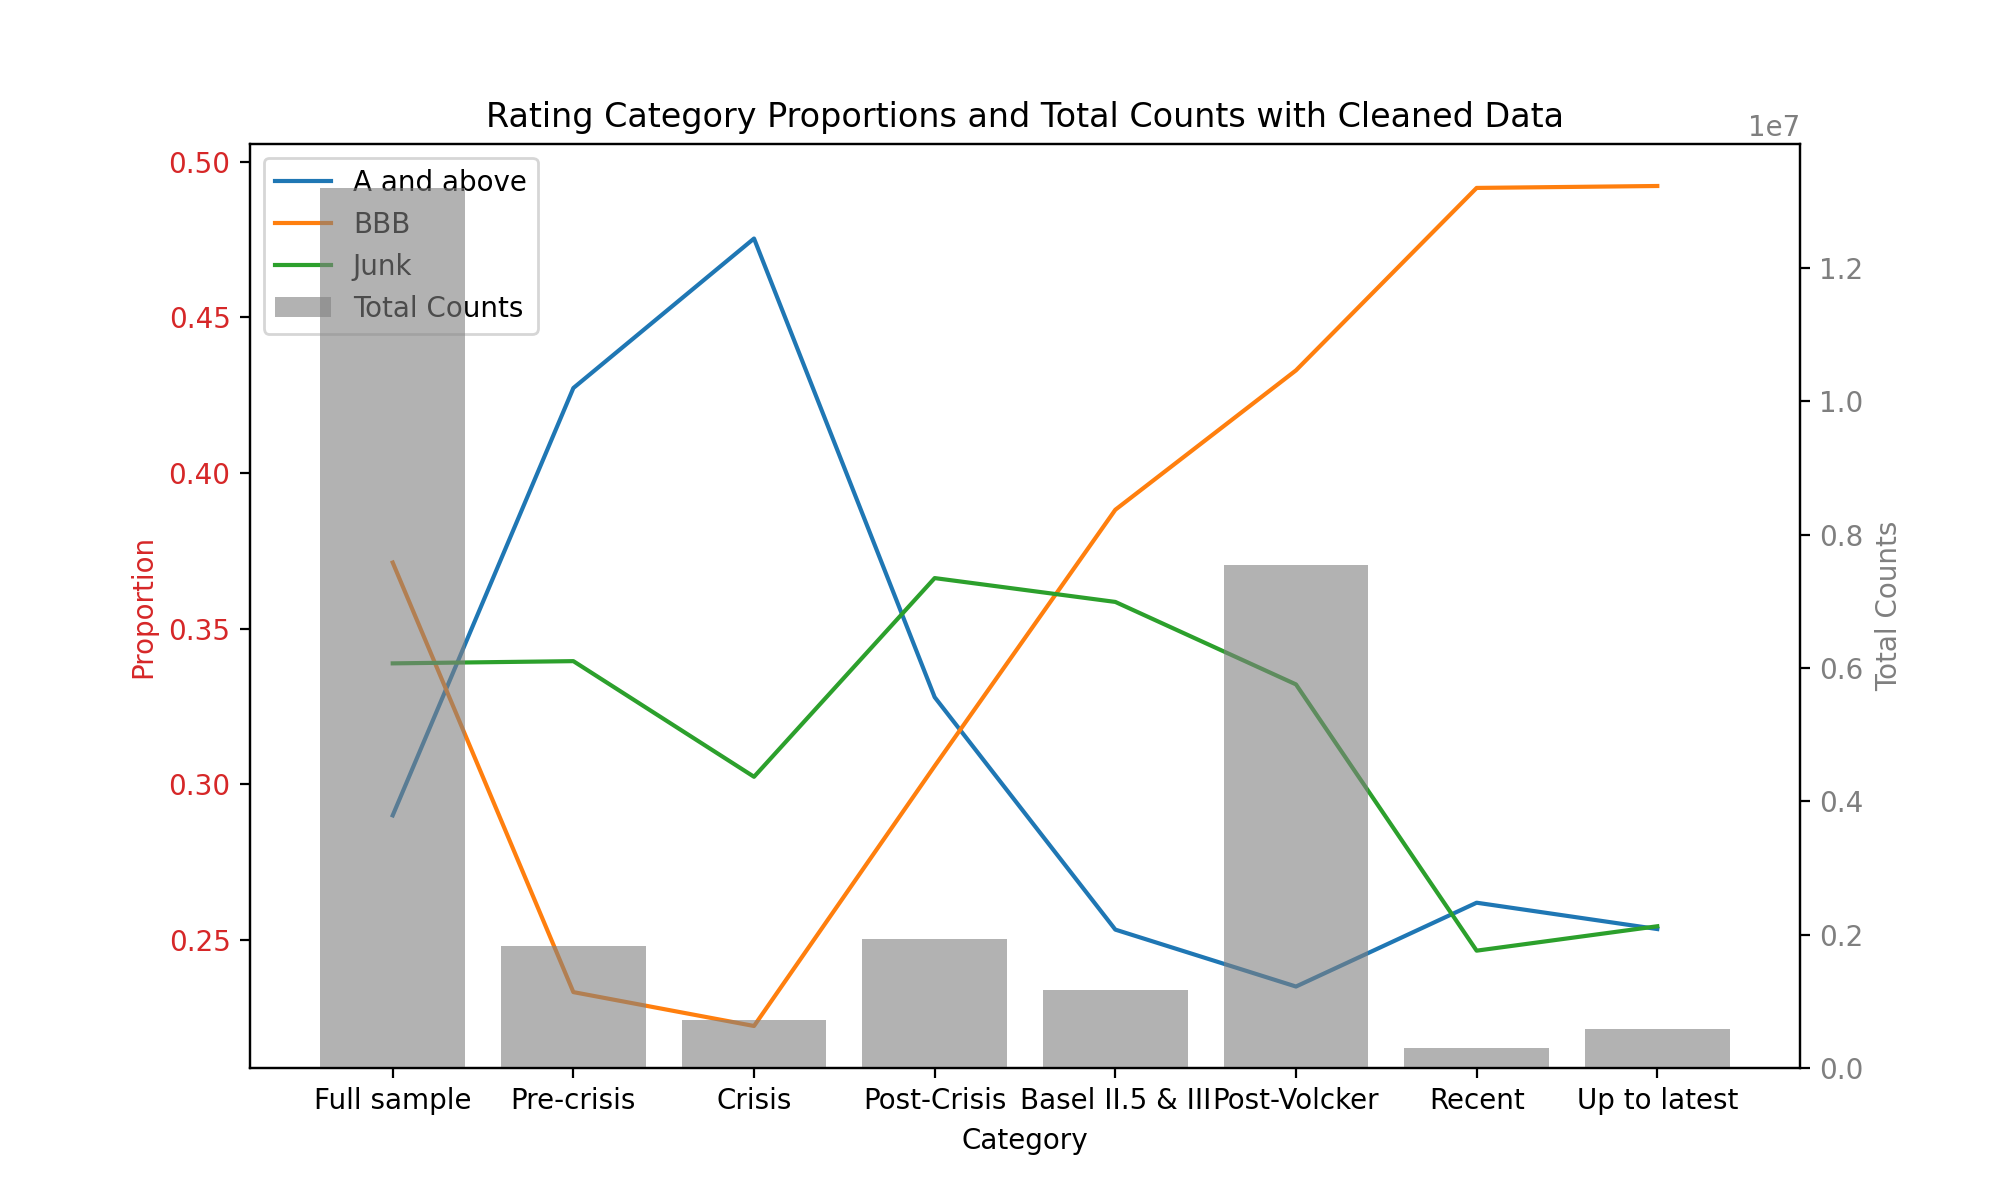
\includegraphics[width=0.75\textwidth]{\PathToOutput/rating_cleaned.png}

% \centering
% 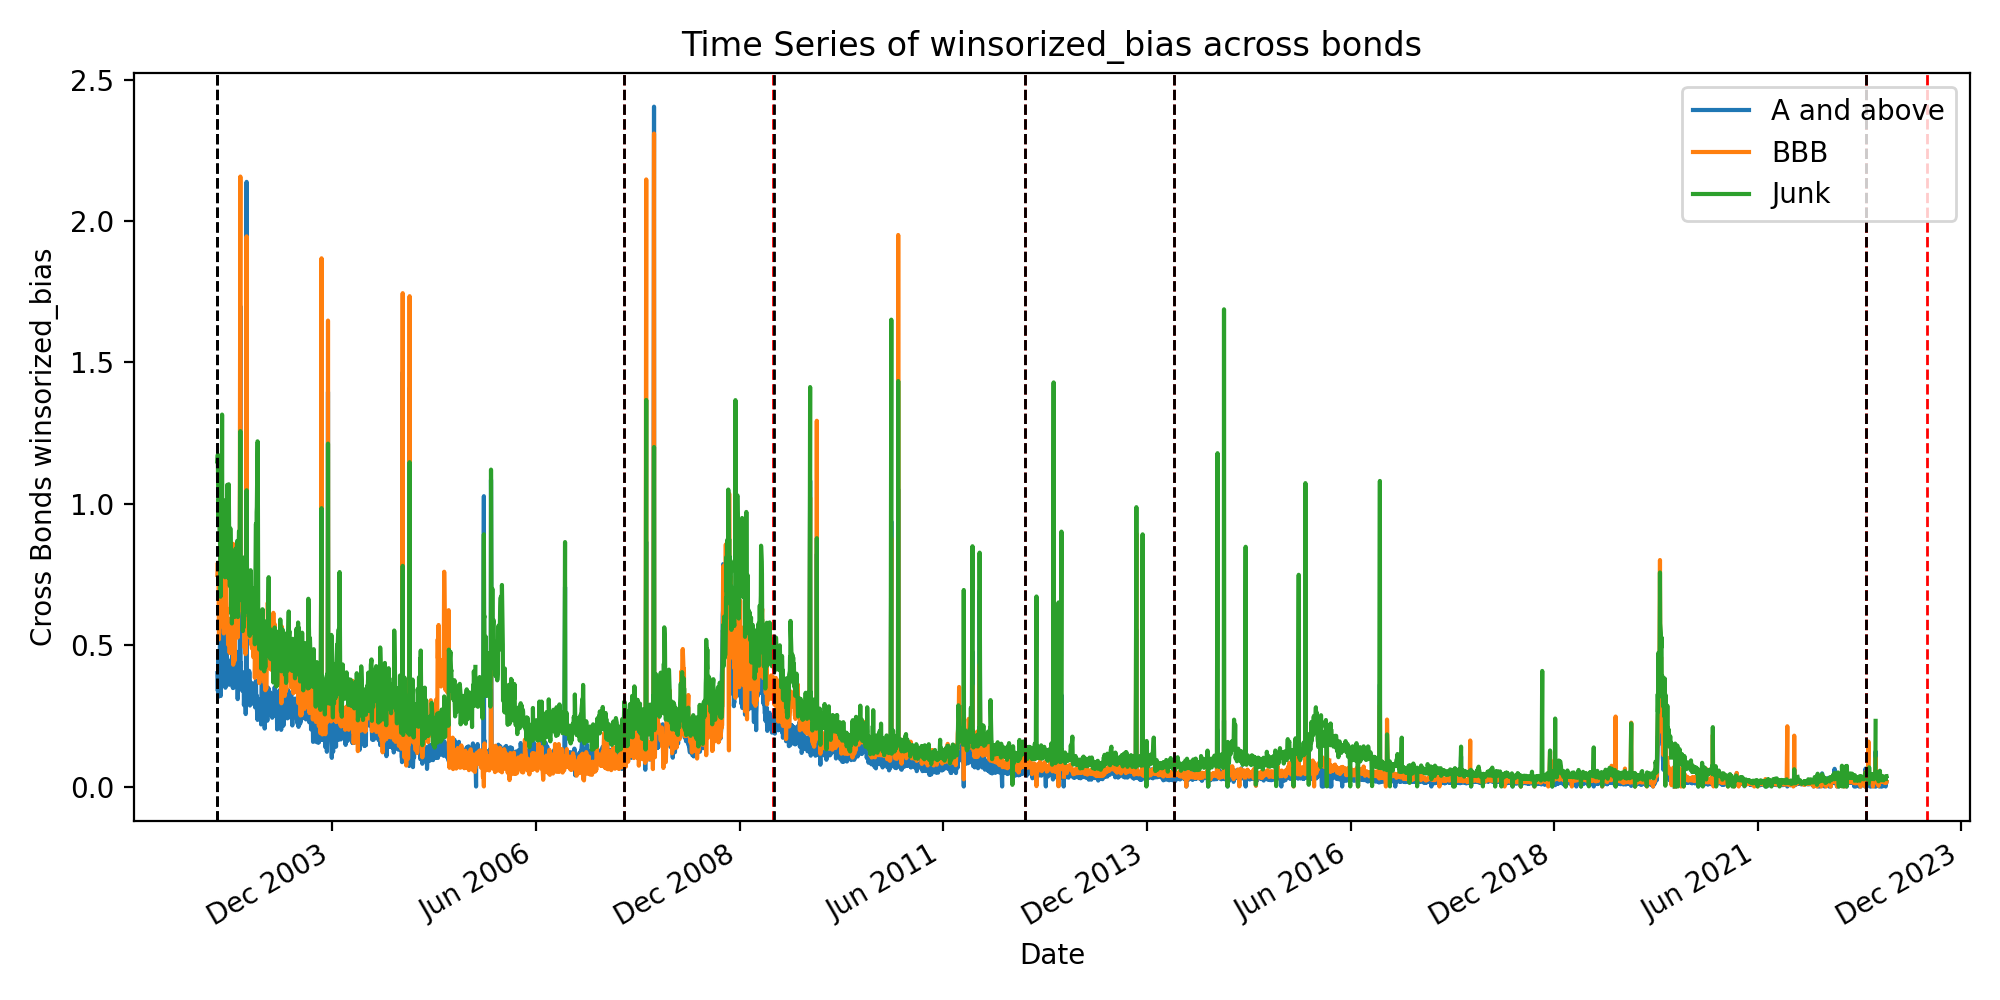
\includegraphics[width=0.75\textwidth]{\PathToOutput/winsorized_bias_categorized.png}
% \caption{\label{fig:myplot}winsorized_bias_categorized}

\section{Results}
\begin{table}[ht]
\centering
\begin{tabular}{llrrrr}
\toprule
 &  & All & A and above & BBB & Junk \\
category & variables &  &  &  &  \\
\midrule
\multirow[t]{4}{*}{Full sample} & Bid-ask bias bps & 0.104 & 0.089 & 0.080 & 0.142 \\
 & Daily return bps & 1.124 & 0.188 & 0.625 & 2.471 \\
 & Bid-ask spread bps & 28.824 & 25.735 & 24.593 & 36.102 \\
 & Credit spread bps & 328.568 & 113.368 & 170.037 & 686.437 \\
\cline{1-6}
\multirow[t]{4}{*}{Pre-crisis} & Bid-ask bias bps & 0.252 & 0.173 & 0.271 & 0.337 \\
 & Daily return bps & 1.971 & -0.342 & -0.602 & 6.649 \\
 & Bid-ask spread bps & 50.196 & 38.798 & 52.971 & 62.633 \\
 & Credit spread bps & 366.367 & 88.509 & 202.033 & 828.895 \\
\cline{1-6}
\multirow[t]{4}{*}{Crisis} & Bid-ask bias bps & 0.305 & 0.243 & 0.324 & 0.389 \\
 & Daily return bps & -1.970 & -0.462 & 6.146 & -10.307 \\
 & Bid-ask spread bps & 59.764 & 53.919 & 60.375 & 68.500 \\
 & Credit spread bps & 745.160 & 283.719 & 570.519 & 1598.856 \\
\cline{1-6}
\multirow[t]{4}{*}{Post-Crisis} & Bid-ask bias bps & 0.149 & 0.106 & 0.148 & 0.187 \\
 & Daily return bps & 7.140 & 3.959 & 5.661 & 11.224 \\
 & Bid-ask spread bps & 39.521 & 33.006 & 39.941 & 45.004 \\
 & Credit spread bps & 491.383 & 163.303 & 250.961 & 985.976 \\
\cline{1-6}
\multirow[t]{4}{*}{Basel II.5 and III} & Bid-ask bias bps & 0.068 & 0.044 & 0.058 & 0.094 \\
 & Daily return bps & 1.639 & 0.171 & 1.312 & 3.031 \\
 & Bid-ask spread bps & 27.013 & 20.285 & 25.221 & 33.706 \\
 & Credit spread bps & 301.945 & 103.300 & 176.851 & 577.699 \\
\cline{1-6}
\multirow[t]{4}{*}{Post-Volcker} & Bid-ask bias bps & 0.042 & 0.024 & 0.033 & 0.068 \\
 & Daily return bps & -0.403 & -0.795 & -0.492 & -0.011 \\
 & Bid-ask spread bps & 18.234 & 12.847 & 16.274 & 24.602 \\
 & Credit spread bps & 242.042 & 75.194 & 130.611 & 505.408 \\
\cline{1-6}
\multirow[t]{4}{*}{Up to latest} & Bid-ask bias bps & 0.102 & 0.088 & 0.078 & 0.140 \\
 & Daily return bps & 1.185 & 0.242 & 0.734 & 2.495 \\
 & Bid-ask spread bps & 28.476 & 25.435 & 24.239 & 35.792 \\
 & Credit spread bps & 324.908 & 112.706 & 168.954 & 680.330 \\
\cline{1-6}
\bottomrule
\end{tabular}

\caption{Replication of Table 1 from the Paper}
\label{tab:derived_table}
\end{table}

\subsection{Comparison with Original Work}
Comparing our replicated table (see Table 2: Replication of Table 1 from the Paper) to the original study's result, our results are off but not in a significant level. We concluded the reasons that we cannot perfectly replicate the figures:

\begin{enumerate}
    \item \textbf{Varying Approaches Yield Divergent Outcomes}. The paper lacks comprehensive details necessary for replicating the process, allowing for a degree of subjectivity in data loading and analytical methods.
    \item \textbf{Utilization of an Outdated Dataset}. The dataset employed in our replication may be more current than the one used by the original authors. It is plausible that the WRDS and TRACE databases have since updated their historical records, potentially excluding anomalies or erroneous bond data. Consequently, the discrepancy in datasets could account for the variations in our results compared to the original study.
    \item \textbf{Exclusion of Maturity Information in the Filtering Criteria}. Our data filtering process omitted consideration of bond maturities. Despite implementing the three specified filtering conditions from section 2.1, we overlooked the criterion that mandates the exclusion of bonds with maturities under one year.
\end{enumerate}



\section{Discussion}

\subsection{Successes}
    Although the replication process was demanding, we achieved several significant milestones:
    \begin{enumerate}
    \item We successfully replicated Table 1, with figures that closely align with the original results.
    \item We gained a comprehensive understanding of the methodologies used to calculate various bond metrics.
    \item We thoroughly examined the authors' coding process by reviewing their GitHub repository.
    \item We met all the requirements set forth by the FINM 32900 Final Project, ensuring that our project was thorough, comprehensive, and well-documented.
\end{enumerate}


\subsection{Challenges}
Although our replication did demonstrated our solid understanding of the paper, we encounter many challenges and we managed to address most of them. 

\begin{enumerate}
    \item \textbf{Absence of Access to a Database System.} One prominent issue involved the handling of large datasets, where conventional methods such as basic Python or pandas read operations proved to be time-consuming.
    \item \textbf{Hardware Inefficiency.} Personal laptops are used for the entire replication process, which is less efficient compared to industrial level hardware. Especially when constructing daily return and credit spread, the original code crashed the kernel on the laptop. Our replication process would be much smoother with more efficient processing tools accessible.
    \item \textbf{Imprecise Analysis.} Given the limited time to finish this project, we only have about two weeks downloading the dataset and replicating the table. The original authors omitted certain steps that, although seemingly trivial, necessitate experimental adjustments and independent exploration on our part. The restricted time frame limits our ability to ensure the utmost accuracy of our results. If more time allowed, the result would be more precise.
    \item \textbf{Time Cost for Each Step.} The efficiency of each step is constrained by limited data sources and hardware resources, impacting our ability to download and process data swiftly. The initial steps of downloading the data and generating return and credit spread alone consume nearly an entire day. This significantly slows the progress of the project.
\end{enumerate}







\section{Conclusion}
In conclusion, our project to replicate Table 1 from "Noisy Prices and Return-based Anomalies in Corporate Bonds" was met with both successes and challenges, which provided invaluable learning experiences. Our replication closely mirrored the original results, affirming the robustness of the methodologies employed by Dickerson, Robotti, and Rossetti. Despite encountering certain obstacles, such as data discrepancies due to updates and the absence of detailed replication guidelines, our endeavor demonstrates that with meticulous methodology and diligent effort, critical academic findings can be substantiated.



% To use BibTeX, include your .bib file name in the bibliography command

\bibliography{bibliography}

\end{document}
